\chapter{Grundlegendes Konzept}

\section{Aufbau einer Webanwendung}
\label{cha:webapplication_structure}

Das Konzept der Schichtenarchitektur ist in der Softwareentwicklung eine Client-Server-Architektur, welche die Darstellung, Anwendungslogik und Datenverwaltung physikalisch trennt.  
Das Konzept der abgestuften Architektur bei der Anwendungsentwicklung lässt sich von einem 1-Stufen-Ansatz bis hin zu einem n-Stufen-Ansatz einteilen. Jeder dieser Ansätze hat seine Vorzüge, doch für eine webbasierte Anwendung eignet sich der n-Stufen-Ansatz. Das Grundkonzept einer solchen Architektur besteht darin, eine Anwendung in unabhängige Ebenen mit definierten Rollen aufzuteilen.
Die mehrstufige Anwendungsarchitektur ermöglicht es den EntwicklerInnen flexible, wiederverwendbare und austauschbare Anwendungskomponenten zu erstellen, welche zu einer Schichtenanwendung verknüpft werden können.
Diese mögen sich auf derselben Maschine befinden, werden aber meist auf unterschiedliche ausgelagert \cite{wiki-ntier-architecture}.

Beispielsweise sind bei dem 1-Stufen-Ansatz alle für die Anwendung relevanten Funktionen -- Darstellung, Logik, Datenverwaltung, \etc -- auf der Clientmaschine vereint. Durch die Limitierung, dass die komplette Software auf einem Gerät betrieben wird, und die daraus folgenden Skalierungsprobleme, ist dieser Ansatz kaum für Webanwendungen geeignet.
Der gebräuchlichste Stufenansatz ist der 3-stufige, siehe Abb.~\ref{fig:3-stufen-architektur}, welcher in der Regel die Darstellung, Anwendungslogik und Datenverwaltung entkoppelt. Ein Webbrowser, zur Anzeige der Benutzeroberfläche, wäre zum Beispiel die erste Stufe. Ein Webserver, welcher die Logik ausführt, repräsentiert die Zweite. Und als dritte Stufe, zur Datenverwaltung, käme eine Datenbank infrage. 

Obwohl der 3-Stufen-Ansatz die Skalierbarkeit erhöht und eine Trennung der Anwendungslogik von den Anzeige- und Datenverwaltungsschichten einführt, trennt er die Anwendung nicht wirklich in spezialisierte Schichten. Für Prototyp- oder einfache Webanwendungen kann eine dreistufige Architektur ausreichen. Bei komplexen Anforderungen an solche Anwendungen ist ein 3-stufiger Ansatz jedoch in mehreren Schlüsselbereichen, einschließlich Flexibilität und Skalierbarkeit, unzureichend, und es wäre sinnvoll, einen n-Stufen-Ansatz zu wählen \cite{nTier-architecture}.

Der größte Nachteil von diesen Ansätzen ist der zusätzliche Overheadaufwand und eine höhere Latenz, was wiederum die der NutzerInnen wahrgenommen Geschwindigkeit mindert.

Die Trennung von Logik ist in der Webentwicklung ein wesentliches Konzept. Wie in diesem Kapitel die Abstraktion durch Stufen, oder Ebenen, wird im folgenden Kapitel \ref{cha:component_usage} die Trennung von Logik, mittels Komponenten, behandelt.

\begin{figure}
	\centering
	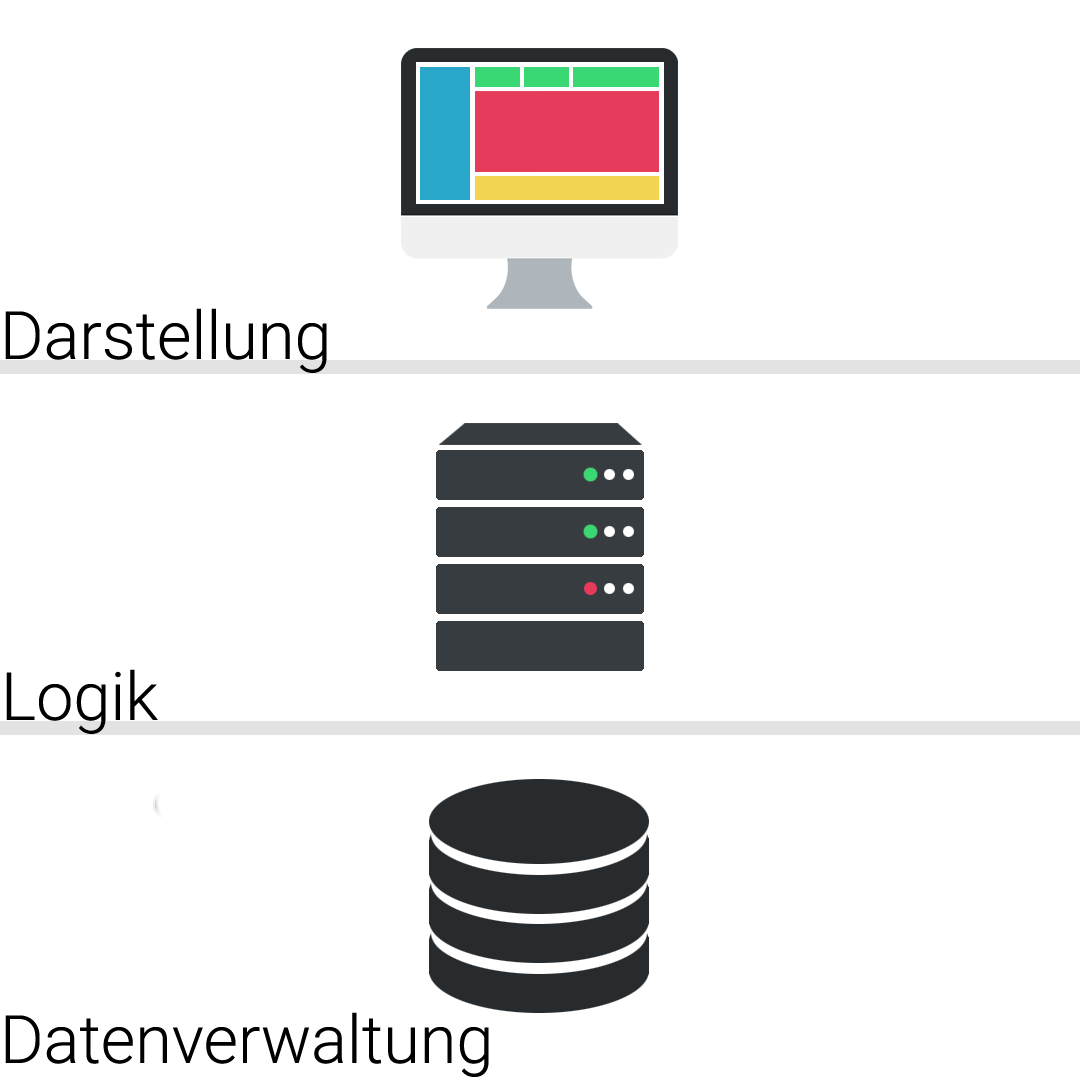
\includegraphics[width=0.5\linewidth]{images/3-stufen-architektur}
	\caption{3-Stufen-Architektur}
	\label{fig:3-stufen-architektur}
\end{figure}

\section{Verwendung von Komponenten im Web}
\label{cha:component_usage}

Das Web besteht aus Bausteinen, sogenannten Elementen. Wenn EntwicklerInnen beispielsweise einen Link mittels einem a-Tag nutzen, wird erwartet, dass dieser sich wie ein Link-Element verhält. Dieses Element hat seine standardmäßige blaue Farbe, einen Handzeiger, wenn sich die Maus über diesem befindet und vor allem die Funktionalität, dass bei einem Klick auf das Element zu einer neuen URL weitergeleitet wird. Dieses Verhalten und Styling wird ohne jegliches Einwirken der EntwicklerInnen bereitgestellt. Jedes HTML-Element funktioniert nach diesem Prinzip, welches HTML Code einfacher zu schreiben und verständlicher macht.
Durch Kombination solcher Elemente, mit eigens definierten Stylesheets können komplexe Gerüste aus HTML-Elementen, mit komplexem CSS/Javascript entstehen.

Damit EntwicklerInnen nicht die komplette Struktur im Kopf behalten müssen, und bei Problemen nur diese, das aufgetretene Problem beheben können, hat es sich bewehrt, Code in kleine, überschaubare Teile herunter zu brechen. In Einheiten, welche das gesamte Gerüst wartbar machen. Diese Teile können einfachere Funktionen, Module, Komponenten oder viele andere Ansätze sein, welche Systeme in atomare Einzelteile aufteilen \cite{components-benefit}.

Komponentenbasierende UI Bibliotheken waren der Standard, um komplexe Anwendungen zu bauen und moderne Webframeworks wie Angular oder Vue ermöglichen den EntwicklerInnen die Nutzeroberfläche aus wiederverwendbaren Blöcken zusammenzusetzen. Der große Unterschied zwischen diesen Frameworks und Webkomponenten ist, dass Webkomponenten die Komponentisierung auf dem DOM-Level durchführen, sodass Custom-Elemente ohne ein Framework, wie Standard HTML-Elemente genutzt werden können. 

Um also die Definition der, in dieser Arbeit fokussierten Technologie -- einer Webkomponente -- zusammenzufassen: Eine entkoppelte Sammlung von Funktionalität oder Prozessen und Logik, mit einer verständlichen Schnittstelle oder API um der Komponente Funktionalität abzurufen.


\section{Eigene Idee, technisches Design}
Durch den Webkomponenten-Standard wird es möglich sein, Komponenten ausschließlich zur Erstellung einer Webanwendung zu nutzen. Um die Grenzen der Nutzung von herkömmlichen Webkomponenten zu überschreiten, und die Verwendung auszuweiten, entwickelte sich die Idee, Webkomponenten gänzlich, oder Teile des Standards, zum Schreiben von CRUD-Anwendungen, und wie in Kap.~\ref{cha:webapplication_structure} erwähnt, die einzelnen Schichten durch Webkomponenten zu realisieren, oder mit den Ebenen durch diese Technologie zu kommunizieren. Sozusagen sollen die Schichten -- Darstellung, Logik, Datenverwaltung -- , welche in Abb.~\ref{fig:3-stufen-architektur} gezeigt sind, mit Webkomponenten realisiert werden. 

\paragraph{Darstellung:}Für diese gibt es bereits konkrete Ansätze und zahlreiche, vorgefertigte Komponenten zur Wiederverwendung\footnote{https://www.webcomponents.org/}.

\paragraph{Logik: }Die Umsetzung der Logik mit Webkomponenten ist noch nicht zur Gänze möglich, da diese im Grunde "`nur"' eine abgekapselte Schicht aus Custom-Elements auf reinen Javascript Code setzen. Ebenso abhängig ist die Realisierung von dem gewählten Technologie Stack. Da das Web bevorzugt Javascript unterstützt, wird auch eine reine Javascript Serverumgebung, beispielsweise Node.js\footnote{https://nodejs.org/}, empfohlen. Jedenfalls gibt es durch die Scram-Engine\footnote{https://github.com/scramjs/scram-engine}, welche in Kap.~\ref{cha:scram-engine} genauer behandelt wird, die Möglichkeit, HTML mit dessen Javascript serverseitig, außerhalb des Browsers, zu parsen, auszuführen und zu rendern. Dadurch werden das Aufsetzen und das Betreiben von Servern, durch die Nutzung von Webkomponenten, ermöglicht.

\paragraph{Datenverwaltung}Diese Schicht per se durch Webkomponenten zu realisieren ist genau so weit möglich, wie die der Logikschicht. Es kann ein Gerüst aus Custom-Elements über die Datenbank Zugriffsschicht gelegt werden, um so Datenbankabfragen mittels Webkomponenten zu tätigen und weiter zu verarbeiten. 


\section{Anforderung an die komponentenorientierte Webanwendung}
Um nun den Grundgedanken der Webkomponenten zu vertiefen, und diese Technologie ausschließlich zur Erstellung einer CRUD-Anwendung zu nutzen, werden folgende Anforderungen gestellt, gruppiert nach Stufen:

\subsection{Darstellung}
Die Anwendung soll eine rudimentäre Benutzeroberfläche zur Verfügung stellen, um alle CRUD-Operationen dem Benutzer zu ermöglichen. 
Für das Erstellen soll ein Formular das Eingeben und Bestätigen von Daten ermöglichen.
Das Auflisten aller vorhandenen Datensätze in einer Tabelle gewährleistet das Lesen.
Ein Formular, wie beim Erstellen, soll mit den Daten des spezifischen Datensatzes ausgefüllt sein, und das Aktualisieren dem Benutzer überlassen.
Das Löschen soll über einen einfachen Auslöser machbar sein.
\subsection{Logik}
So weit es die Webkomponenten zulassen, soll der Server mit diesen strukturiert und konfiguriert werden.

\subsection{Datenverwaltung}
Die Interaktion mit der Datenbank soll durch Webkomponenten das Erstellen, Lesen, Aktualisieren und Löschen eines Datensatzes ermöglichen. Das bedeutet, alle CRUD-Operationen sollen durch Webkomponenten ausführbar sein. 

